\documentclass[tikz,border=10pt]{standalone}
\usepackage{pgfplots}
\usepackage{tikz}
\usepackage{amsmath}

\begin{document}

\begin{figure}
    \centering
    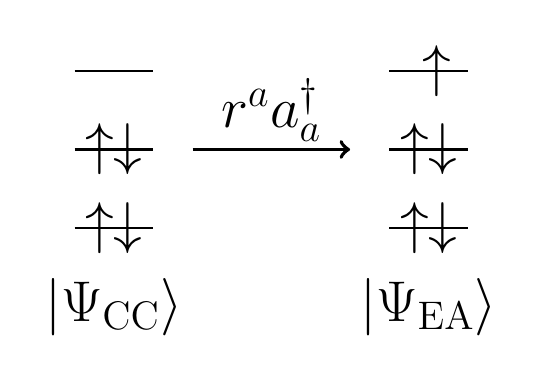
\begin{tikzpicture}
        \huge
        % Define styles
        \tikzset{
            level/.style={thick},
            arrow/.style={->, thick},
            label/.style={font=\small}
        }

        % Draw CC wavefunction levels (left)
        \draw[level] (-2,2) -- (-1,2); 
        \draw[level] (-2,1) -- (-1,1);
        \draw[level] (-2,0) -- (-1,0);
        
        % Draw electron occupancies for CC
        \node at (-1.5,0) {\(\uparrow\downarrow\)};
        \node at (-1.5,1) {\(\uparrow\downarrow\)};

        % Label CC wavefunction
        \node[label] at (-1.5,-1) {\huge\(|\Psi_{\text{CC}}\rangle\)};

        % Draw EA wavefunction levels (right)
        \draw[level] (2,2) -- (3,2);
        \draw[level] (2,1) -- (3,1);
        \draw[level] (2,0) -- (3,0);
        
        % Draw electron occupancies for EA
        \node at (2.6,2) {\(\uparrow\)};
        \node at (2.5,0) {\(\uparrow\downarrow\)};
        \node at (2.5,1) {\(\uparrow\downarrow\)};

        % Label EA wavefunction
        \node[label] at (2.5,-1) {\huge\(|\Psi_{\text{EA}}\rangle\)};

        % Draw transition arrow and label
        \draw [->,line width=0.5mm] (-0.5,1) -- (1.5,1);
        \node[label] at (0.5,1.5) {\huge\(r^a a^\dagger_a\)};
    \end{tikzpicture}
\end{figure}

\end{document}
